The perceptron of section \ref{subs:perceptron} can be considered as a linear classifier for which the decision boundary is the hyperplane
$$ b + w_1 \cdot x_1 + ... + w_n \cdot x_n = 0$$
It is limited because it has only a linear boundary. To have a non-linear model, we can have multiple perceptron giving multiple outputs. This layer of perceptron is called a \acrfull{fcn} and is illustrated at figure \ref{fig:fcn}.
\begin{figure}[h]
    \centering
    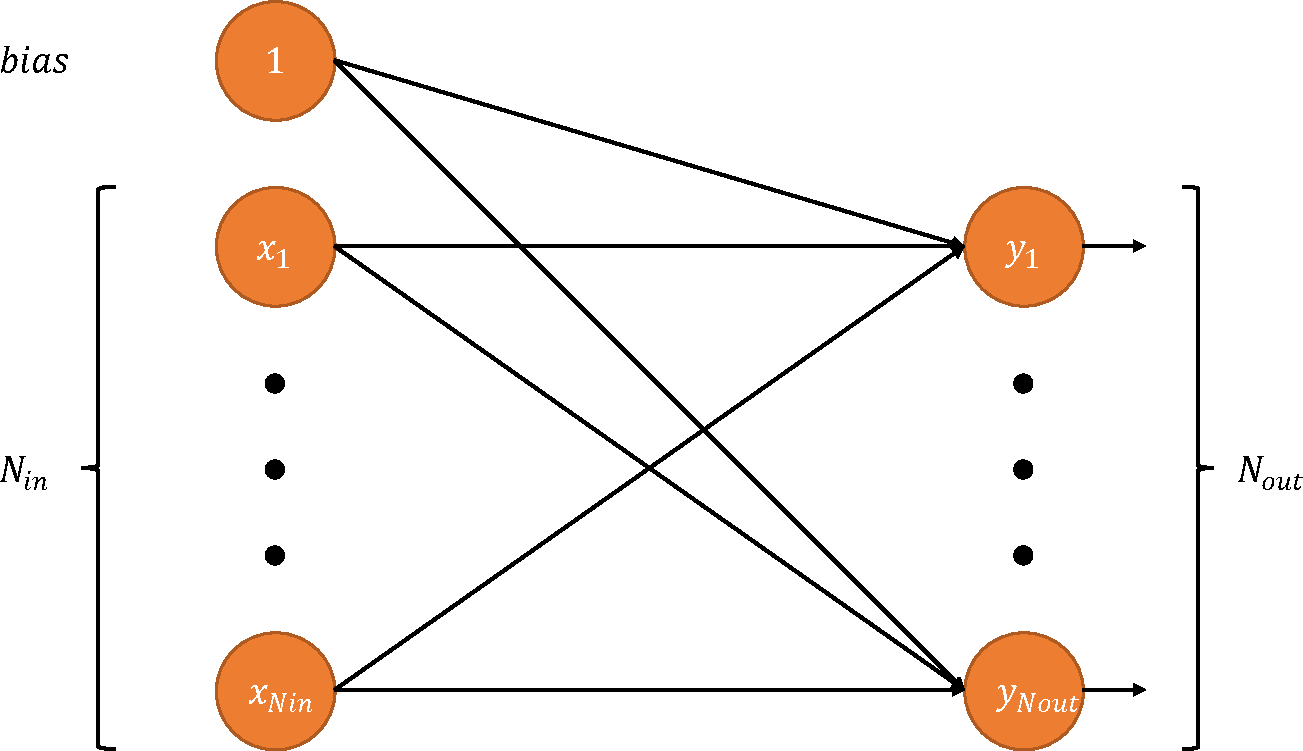
\includegraphics[width=\textwidth]{Images/fcl.pdf}
    \caption{A fully connected layer}
    \label{fig:fcn}
\end{figure}
